% Worksheet
% NOTE: For two marks complete and hand-in Pages 7-8 before the end of the lab.
% You are a design engineer working at a large automotive component manufacturer. You 
% have been asked to design a system to monitor the air intake filter on an engine. You are 
% to devise a system that will determine if the air filter is properly installed or damaged and
% when the filter is clogged, which will turn on the engine warning light, so that the driver 
% knows that the filter will need to be replaced. 
% When a clean filter is installed, the pressure drop across the filter is 0.7 kPa when the 
% engine is at idle. (The pressure drop is the differential pressure between the air upstream 
% and downstream of the filter). If a filter has a leak due to damage or improper installation, 
% then the pressure drop will be lower than 0.7 kPa. For example, the pressure drop will be 
% zero if no filter is installed. Also, as debris is collected on the filter the pressure drop 
% increases. The filter should be replaced when the pressure drop reaches 0.9 kPa when the 
% engine is at idle. Thus, it is desired to measure pressure drops from 0 to 0.9 kPa.
% The analog signal from the pressure transducer will be read by the vehicle’s engine 
% control unit (ECU). The ECU uses a 12-bit A/D converter and accepts 0–5 V input 
% voltage.
% Your supervisor told you to use a sensor from Honeywell (see data sheet posted on 
% eClass) that measures differential pressure with the model number: 
% ABP2 D DA D XXXXX A A Y, where XXXXX is a place holder for the pressure range, 
% and Y is a place holder for the supply voltage (either 3.3 V or 5 V). See Page 10 of the 
% data sheet to understand the model number. 
% Recommend a system to monitor the pressure drop by completing the following steps:
% 1) See Page 10 of the data sheet and select a pressure range in kPa which is 
% suitable for your application. [1 mark]. Why did you choose that range? [1 
% mark].
% 2) See Page 6 of the data sheet. The output of the sensor depends on the supply 
% voltage of the sensor. Plot the expected voltage output of your sensor as a 
% function of pressure over the range of the sensor if the supply voltage is 3.3 V 
% and if it is 5V. Put both lines on the same plot. [2 marks]. Calculate the 
% sensitivity of the sensor for each supply voltage. [1 mark]
% 3) The ECU uses 12-bit A/D converters and has channels which can accept 0–
% 5 V input voltages. Also, it is possible to amplify the signal out of the sensor 
% before it goes to the ECU. For each supply voltage (either 3.3 V or 5 V), 
% calculate the maximum amplification you could use [3 marks] and the 
% resulting resolution of the measurement system in units of kPa [1 marks]
% 4) Read Page 3 and Page 13 of the data sheet. Determine the total bias 
% uncertainty in your system, in units of kPa, for each supply voltage (either 3.3 
% MecE-301 10
% V or 5 V) using maximum amplification when the pressure transducer is 
% measuring 0.9 kPa when used in the temperature range of -20 to 85 oC. [3 
% marks] [Note: There is a bias uncertainty due to resolution of the A/D and a 
% bias uncertainty of the sensor].
% 5) State which supply voltage and amplification (if any) that should be used. [1 
% mark]. Is the cost and complexity of amplification worth the benefit of 
% increased resolution? [1 mark]. Why do you recommend the supply voltage 
% that you did? [1 mark] Is the uncertainty acceptable for this application? Why
% or why not? [1 marks]
% 6) Rapid pressure fluctuations can occur in the engine intake, which may disrupt 
% your measurements. Recommend a method so that these fluctuations do not 
% disrupt your measurement. [1 mark]
% Note: 3 Marks will be given based on the clarity of the presentation of your calculations 
% and discussion

\section{}
% Question 1
Define a list of the design criteria:
\begin{itemize}
    \item Pressure range: 0-9 kPa
    \item Resolution should be maximized since the number of bits is fixed to $2^{24}$
    \item Working unit: kPa
\end{itemize}

One pressure range meets these constraints: $\boxed{\text{001KD}}$.   

\section{}
% qeustion 2 reponse
\begin{figure}[h]
    \centering
    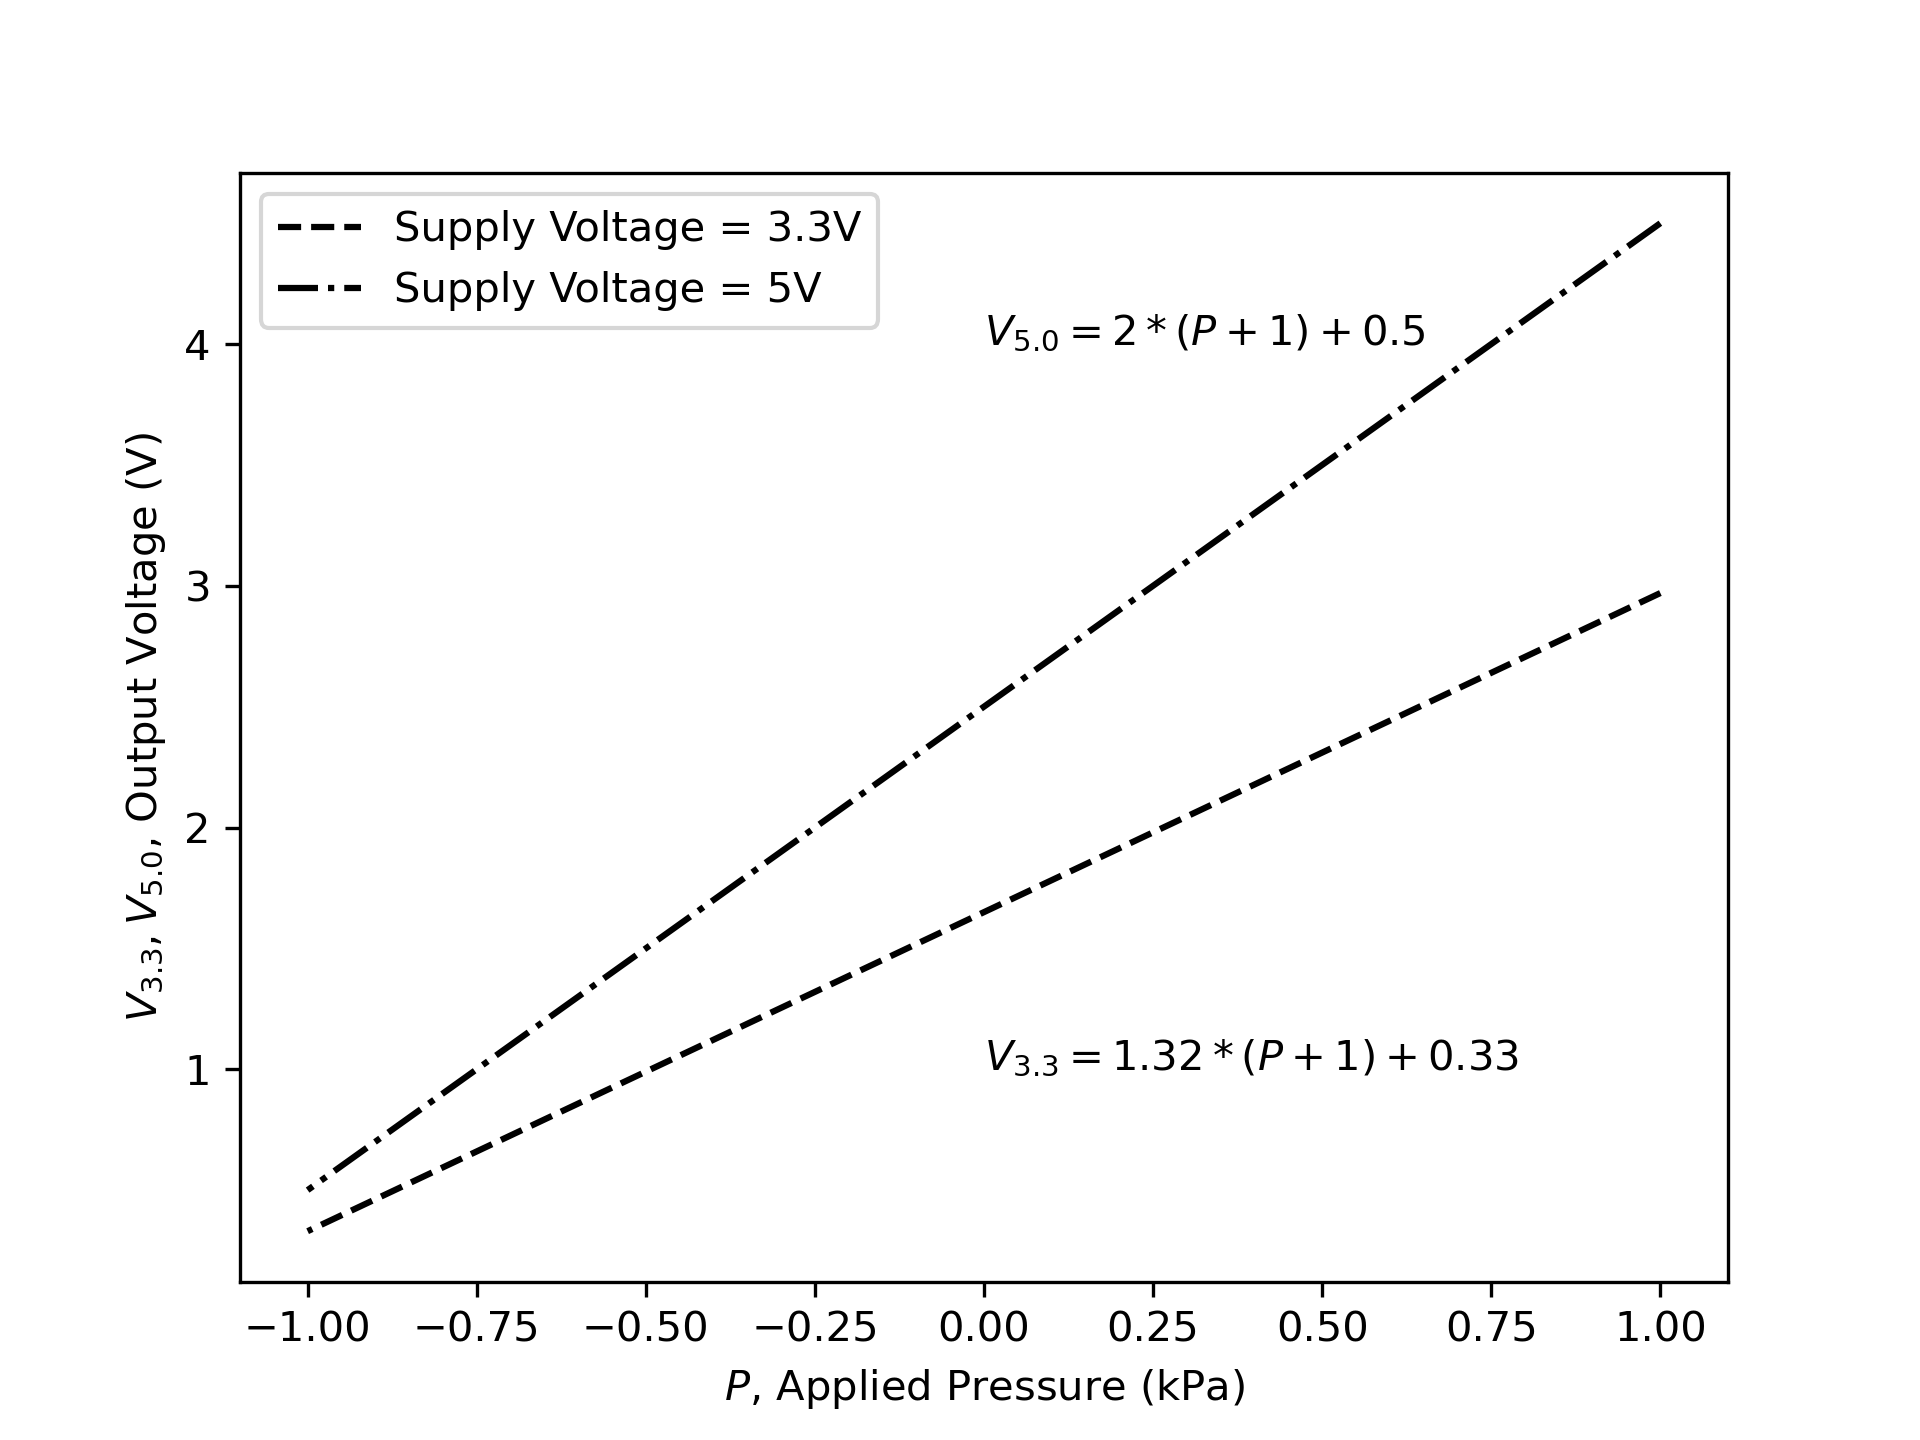
\includegraphics[width=0.8\linewidth]{matplotlib/q2VoltageOutputPlot.png}
    \caption{Voltage output of the sensor as a function of pressure over the range of the sensor if the supply voltage is 3.3 V and if it is 5V.}
    \label{fig:q2VoltageOutputPlot}
\end{figure}
The sensitivity of the sensor for each supply voltage is calculated by taking the derivative of the voltage output with respect to pressure. 
Since the equations for the voltage output are linear, the sensitivity is constant. 
\begin{align*}
    \text{Sensitivity}_{3.3V} &= \frac{d}{dP} \left( 1.32*(P+1) + 0.33 \right) = 1.32 \text{ V/kPa} \\
    \text{Sensitivity}_{5V} &= \frac{d}{dP} \left( 2*(P+1) + 0.5 \right) = 2 \text{ V/kPa}
\end{align*}

% plt.text(0, 1, '$V_{3.3} = 1.32*(P+1) + 0.33$')
% plt.text(0, 4, '$V_{5.0} = 2*(P+1) + 0.5$')

\section{}
The transfer function being used has an output range of 10\% to 90\% of the input range. That means the maximum output of the 
sensor is $0.9V_{\text{input}}$ 

For the 3.3V supply voltage, the highest output from the sensor is $V_{\text{o, max}} = 0.9\times3.3$. The maximum the EDC can read is 5V, so the maximum amplification is:
\begin{empheq}[box=\fbox]{align*}
    \text{Amplification}_{3.3V} &= \frac{V_{\text{EDC, max}}}{V_{o, max}} = \frac{5}{0.9\times3.3} = 1.68
\end{empheq}
For the 5V supply voltage, the highest output from the sensor is $V_{\text{o, max}} = 0.9\times5$. The maximum amplification is:
\begin{empheq}[box=\fbox]{align*}
    \text{Amplification}_{5V} &= \frac{V_{\text{EDC, max}}}{V_{o, max}} = \frac{5}{0.9\times5} = 1.11
\end{empheq}
